\chapter{Diseño}

\section{Diseño de las herramientas}

\subsection{Diseño de la base de datos}
Las diferentes colecciones de la base de datos se han extraído a partir de ficheros existentes dentro de un servidor del Spanish Virual Observatory (SVO) dentro del Departamento de Arquitectura y Tecnología de Sistemas Informáticos de la Escuela Técnica Superior de Ingenieros Informáticos de la Universidad Politécnica de Madrid. 

A partir de estos ficheros CSV se tomó la decisión de crear las siguientes colecciones.


\begin{itemize}
    \item \textbf{Estación}: En esta colección tenemos la información necesaria sobre las estaciones de radiodetección disponibles. En el momento de la realización del trabajo sólo existe una estación trabajando, aunque existe previsión de que en un futuro se adhieran varias más al proyecto. 
        \begin{itemize}
            \item \_id: el identificador de la estación.
            \item Localización: la ubicación donde se encuentra la estación.
            \item web: página web de la estación.
        \end{itemize}
    \item \textbf{Eco}: esta colección contiene los datos de las detecciones.
        \begin{itemize}
            \item \_id: el identificador de la estación.
            \item Fecha: la fecha en la que se produce la detección.
            \item Id\_Estacion: la estación donde se detecta el meteoroide.
            \item Duración: la duración que tiene el eco.
        \end{itemize}
    \item \textbf{Espectrograma}: espectrograma que se genera a partir de los datos del eco detectado.
        \begin{itemize}
            \item \_id: el identificador del espectrograma.
            \item Id\_Estacion: la estación de detección..
            \item Votable: ubicación del fichero votable del espectrograma en el servidor.
            \item Imagen: ubicación de la imagen del espectrograma en el servidor.
            \item Csv: ubicación del fichero csv del espectrograma en el servidor.
        \end{itemize}
    \item \textbf{Curva Luz}: curva de luz que se genera a partir de los datos eco detectado.
        \begin{itemize}
            \item \_id: el identificador de la curva de luz.
            \item Id\_Estacion: la estación de detección.
            \item Votable: ubicación del fichero votable de la curva de luz en el servidor.
            \item Imagen: ubicación de la imagen de la curva de luz en el servidor.
            \item Csv: ubicación del fichero csv de la curva de luz en el servidor.
        \end{itemize}
    \item \textbf{Sonido}: sonido generado a través de la curva de luz
        \begin{itemize}
            \item \_id: el identificador del sonido.
            \item Ruta: localización del fichero de sonido dentro del servidor.
        \end{itemize}
    \item \textbf{Clasificación}: clasificación de un eco, puede provenir del asistente virtual o de la plataforma zooniverse.
        \begin{itemize}
            \item \_id: el identificador de la clasificación.
            \item idUsuario: identificador del usuario que realiza la tarea de clasificación.
            \item Respuesta1: primera respuesta dada por el usuario.
            \item Respuesta2: segunda respuesta dada por el usuario.
            \item Respuesta3: tercera respuesta dada por el usuario.
        \end{itemize}
\end{itemize}


Las tablas las obtenemos desde ficheros que se encuentran en un servidor del Spanish Virual Observatory (SVO) dentro del Departamento de Arquitectura y Tecnología de Sistemas Informáticos de la Escuela Técnica Superior de Ingenieros Informáticos de la Universidad Politécnica de Madrid. A partir de este fichero se crean las tablas que se aprecian en la figura \ref{fig:tablas_base_datos}

\begin{figure}[h]
    \centering
    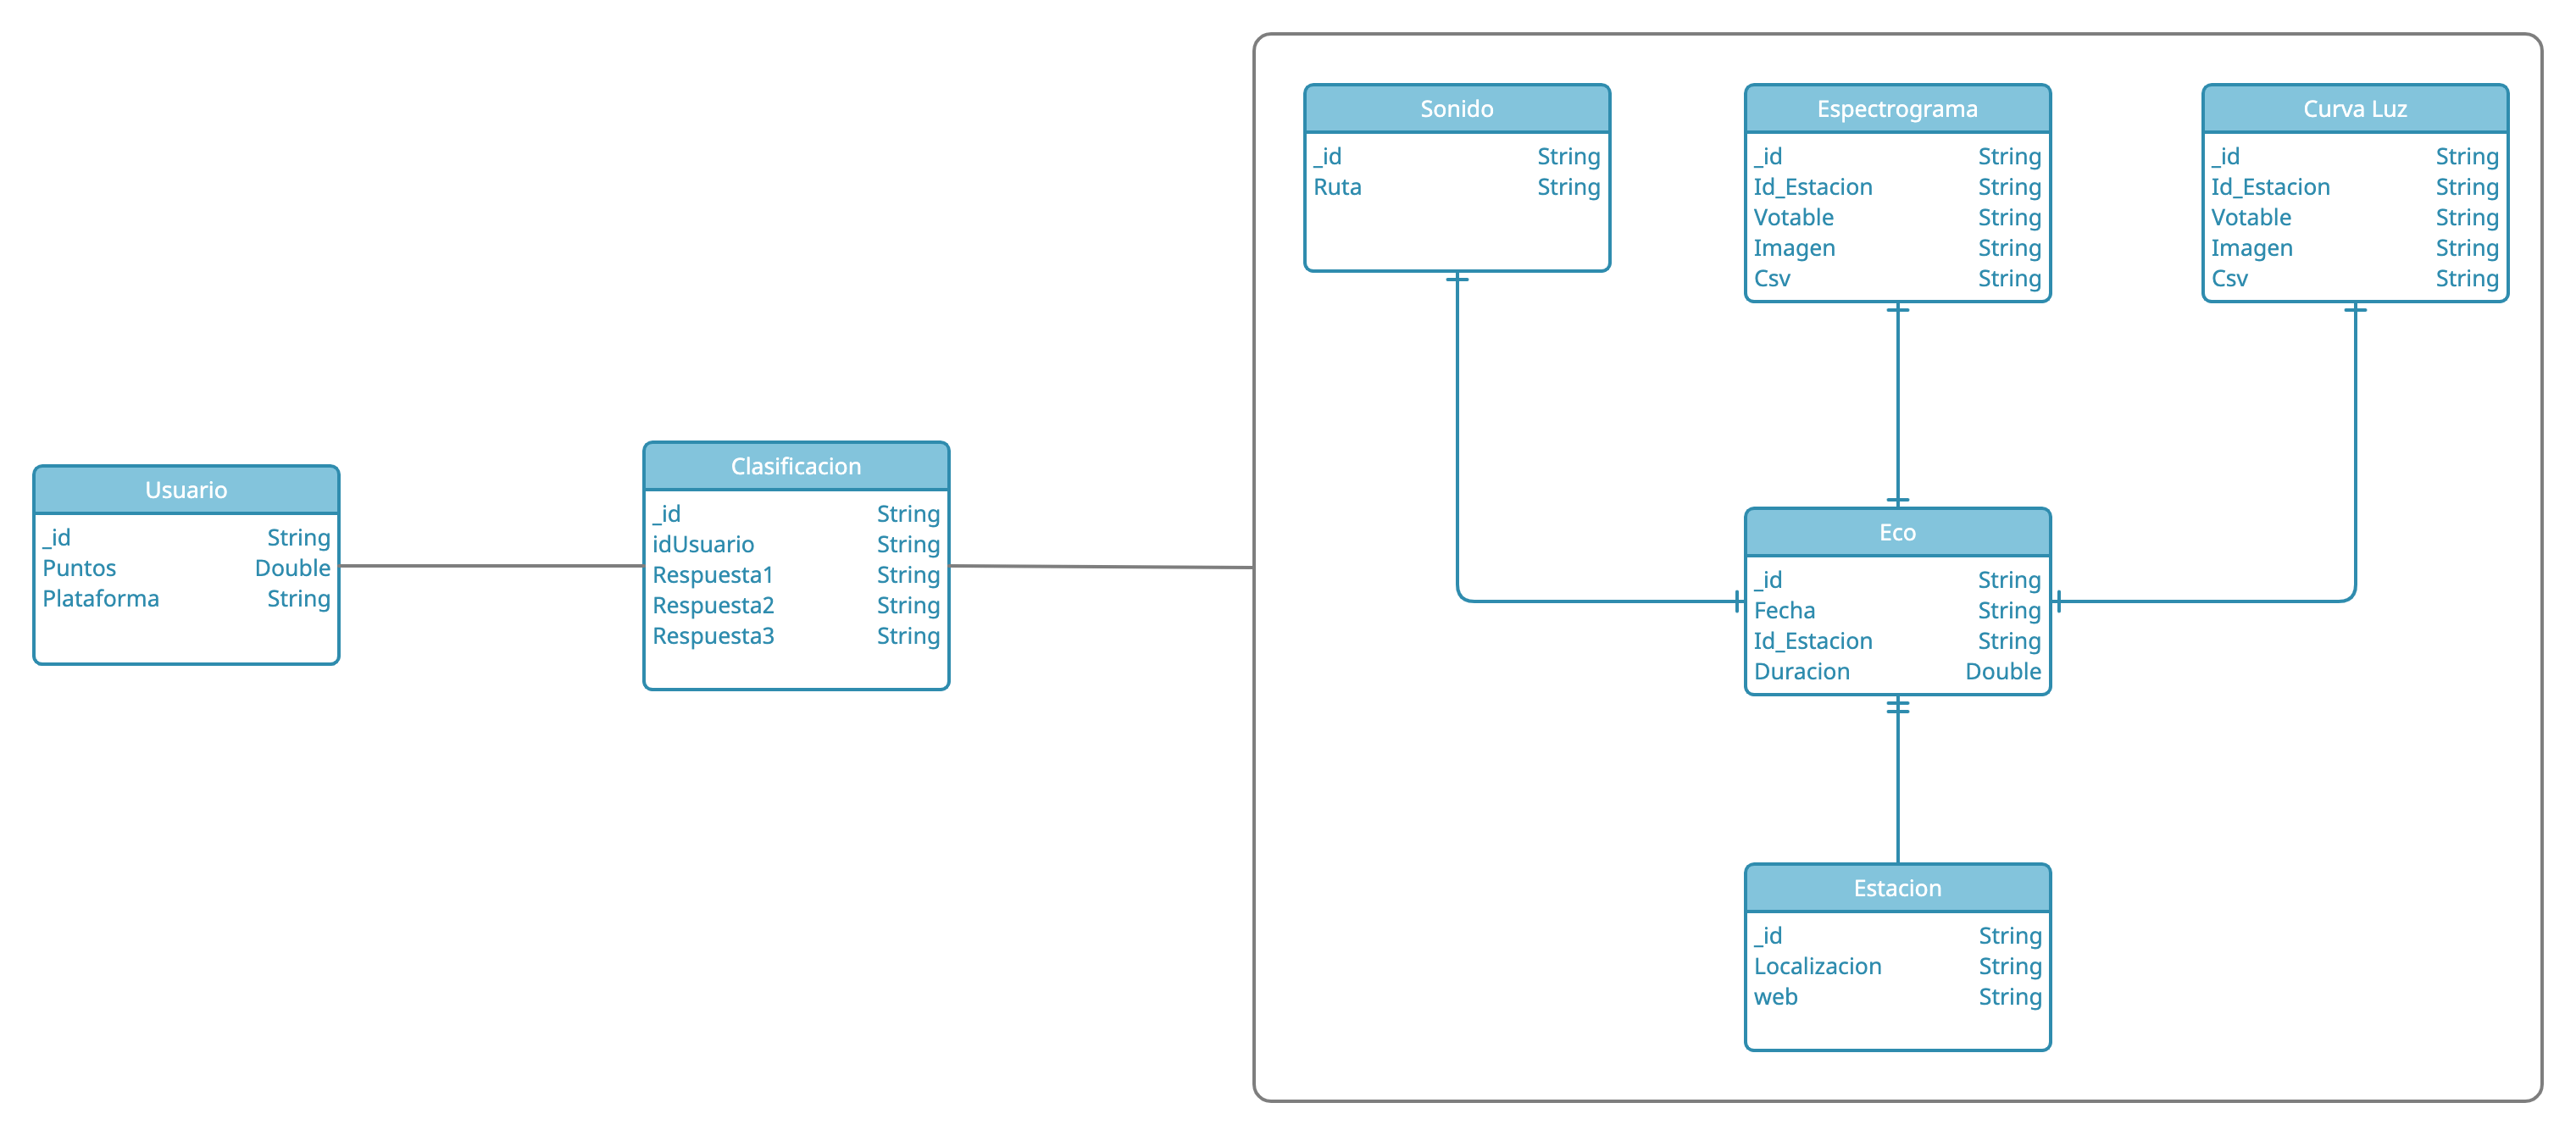
\includegraphics[width=\textwidth]{include/figuras/Tablas.png}
    \caption{Colecciones de la base de datos}
    \label{fig:tablas_base_datos}
\end{figure}

Aunque hemos explicado anteriormente que no es estrictamente necesario que existan relaciones entre las tablas, en este proyecto sí que es necesario, puesto que varias tablas proceden del mismo meteoroide.


\subsection{Estructura de la aplicación RESTful}

\begin{figure}[H]
    \centering
    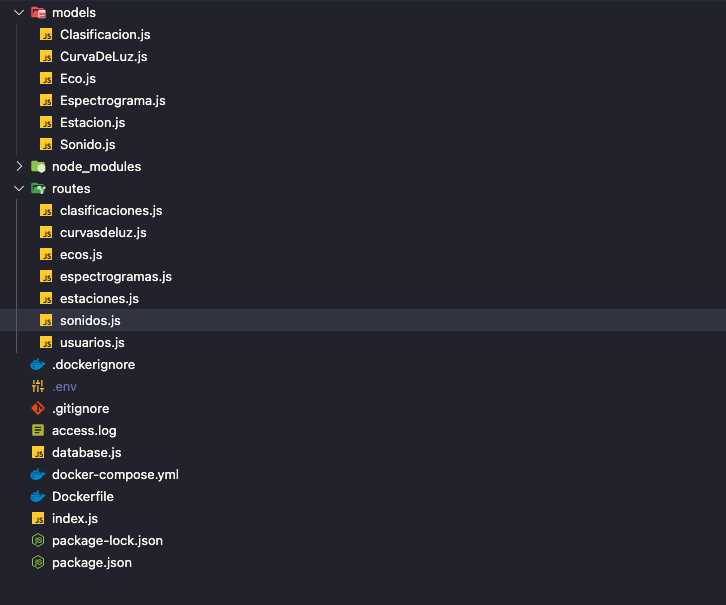
\includegraphics[width=\textwidth]{include/figuras/EstructuraAPI.png}
    \caption{Estructura de la aplicación RESTful}
    \label{fig:estructura_api}
\end{figure}

En esta figura \ref{fig:estructura_api} se observa la estructura que adopta el desarrollo de la API RESTful. A continuación se va a explicar qué es fichero y qué contiene cada carpeta existente en el proyecto.

En la raíz del proyecto tenemos diversos ficheros:

\begin{itemize}
    \item .dockerignore: en este fichero se especifican los ficheros a excluir dentro de un contenedor de docker.
    \item .env: se trata de un fichero en el cual se establecen ciertas variables de entorno. En nuestro caso contiene la cadena de conexión a la base de datos. Se utiliza este fichero para evitar posibles filtraciones de la contraseña en caso de que el código sea compartido en Github o cualquier otra plataforma de colaboración.
    \item .gitignore: fichero con un funcionamiento similar al dockerignore pero destinado a Git y Github.
    \item database.js: se establece la comunicación entre la API REST y la base de datos a través de la cadena de conexión existente dentro del fichero .env.
    \item docker-compose.yml: este fichero se utiliza para el despliegue automático de varios contenedores de manera simultánea, estableciendo entre sí una especie de "red virtual" que permite la conexión entre los distintos contenedores.
    \item Dockerfile: este fichero se utiliza para la generación de una imagen del proyecto que luego se utiliza en el despliegue de un contenedor o dentro de un docker-compose.
    \item index.js: es el fichero principal de la aplicación. En él están definidas la ruta principal de la API, las rutas de los demás controladores, las variables principales de Swagger y la ruta en la que se despliega el servicio.  
    \item package.json: en este fichero están definidas las opciones de los módulos de node.js utilizados en el desarrollo y las principales opciones de nuestra aplicación (nombre, versión, descripción y fichero \textit{main}).
\end{itemize}

En primer lugar se observa la carpeta models. Esta carpeta contiene todos los modelos necesarios de las colecciones existentes en la base de datos. Es necesario definir modelos puesto que el módulo de Node.js que estamos utilizando en el desarrollo de la API nos exige su utilización para un correcto funcionamiento. 

La carpeta node\_modules contiene todos los módulos necesarios para nuestra implementación.

A continuación tenemos la carpeta routes, en ella están definidas todas las rutas que tiene accesible la API y todos las llamadas disponibles (GET,POST,PATCH y DELETE).

\newpage
\subsection{Estructura de la aplicación Rasa}

En la siguiente figura \ref{fig:estructura_chatbot} se muestra cuál es la estructura de la aplicación desarrollada en Rasa.

\begin{figure}[H]
    \centering
    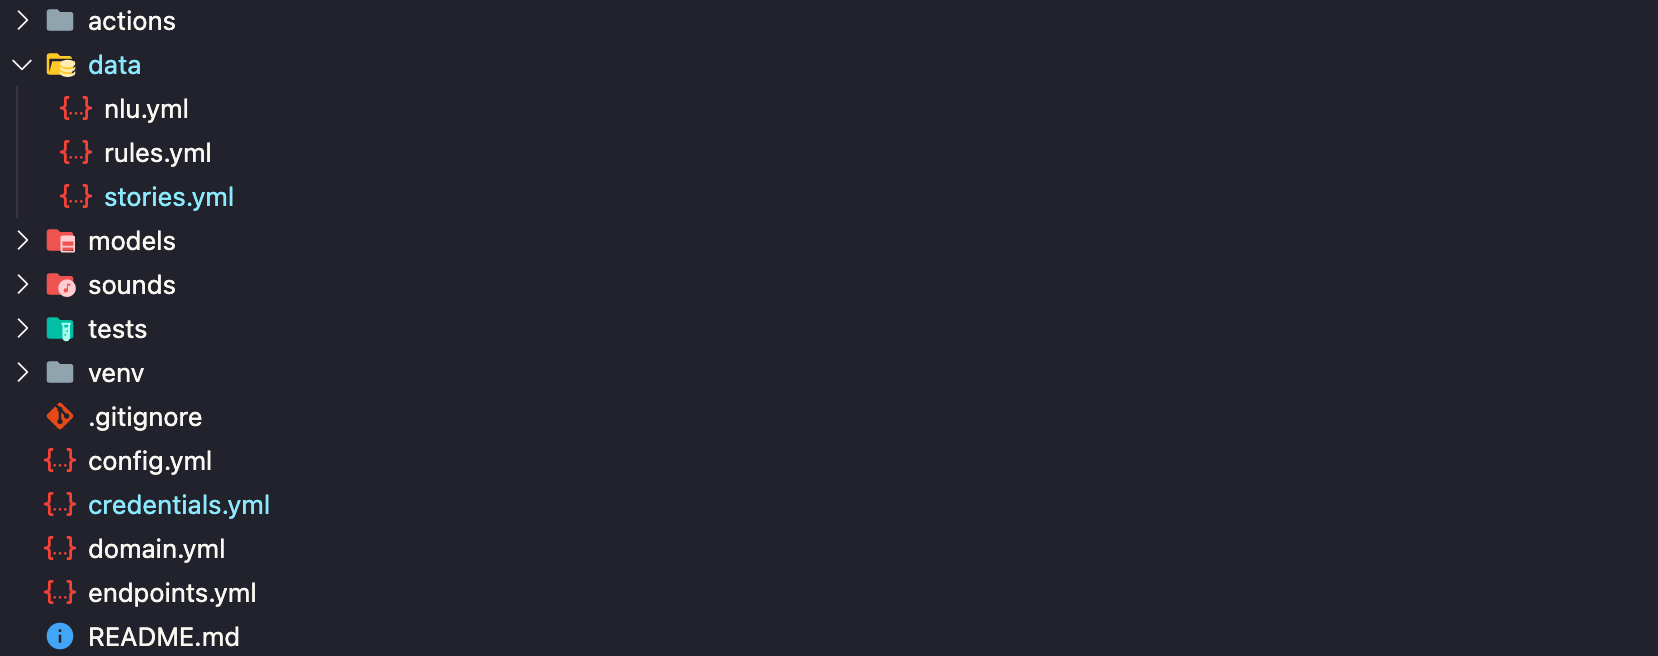
\includegraphics[width=\textwidth]{include/figuras/EstructuraChatbot.png}
    \caption{Estructura del asistente virtual}
    \label{fig:estructura_chatbot}
\end{figure}

Dentro de todos los ficheros y carpetas que se crean al iniciar un proyecto de Rasa se van a explicar todos los elementos necesarios para el correcto desarrollo.

\begin{itemize}
    \item \textbf{Actions}: dentro de esta carpeta el único fichero que necesitamos es el \textit{action.py}. En él se encuentran todas las acciones personalizadas que requiere el proyecto.
    \item \textbf{data}: dentro de esta carpeta se encuentran los ficheros más importantes del módulo NLU (Natural Lenguage Understanding). Estos ficheros son:
    \begin{itemize}
        \item nlu.yml: en este fichero se encuentran los intents definidos por el usuario.
        \item rules.yml: se definen cada una de las posibles reglas a utilizar por el asistente.
        \item stories.yml: en él se desarrollan los diferentes caminos posibles dentro del flujo de diálogo.
    \end{itemize}
    \item \textbf{models}: dentro de esta carpeta se guardan los modelos autogenerados cada vez que entrenamos el chatbot.
    \item \textbf{sounds}: en el interior de esta carpeta se encuentra una muestra de los sonidos disponibles dentro de la base de datos.
    \item \textbf{test}: aquí están los ficheros autogenerados con posibles conversaciones que puede seguir el chatbot.
    \item \textbf{venv}: se trata del entorno virtual en el que se ejecuta el chatbot.
    \item \textbf{.gitignore}: fichero destinado a Git y Github en el cual se especifican los ficheros y carpetas dentro del documento que no se subirán al repositorio.
    \item \textbf{config.yml}: dentro de este fichero de configuración se definen las distintas políticas y distintos componentes que el modelo utilizará para realizar predicciones basadas en las entradas que proporcione el usuario.
    \item \textbf{credentials.yml}: en este fichero se incluyen los diferentes credenciales para conectar Rasa con múltiples servicios.
    \item \textbf{domain.yml}: se trata de uno de los ficheros más importantes del chatbot. Define el universo en el que opera el asistente. Dentro de él se incluyen todos los intents, entities, slots, responses, forms y acciones que el chatbot debe conocer. En él también se incluyen parámetros de configuración de las sesiones del chatbot.
    \item \textbf{endpoints.yml}: se especifican los distintos endpoints a los que se puede conectar el asistente. En nuestro caso sólo se conecta con el servidor en el que se despliegan las acciones.
\end{itemize}

\section{Despliegue de las herramientas}

\subsection{Despliegue del asistente}
Es obligatorio especificar en qué sistema operativo se va a realizar el despliegue de la herramienta. En caso de que se realizase sobre Windows, sería necesario instalar primeramente el lenguaje Python, ya que todo el framework de Rasa está basado en este lenguaje. Si se realiza sobre un sistema Linux o un sistema UNIX no es necesario instalarlo ya que en la mayoría de distribuciones viene instalado por defecto.

Una vez tengamos instalado el lenguaje Python, se crea un entorno virtual como se muestra en la figura \ref{fig:venv}. Esta herramienta nos permite instalar todas las dependencias necesarias para el framework sin comprometer la estabilidad del sistema operativo. 

\begin{figure}[H]
    \centering
    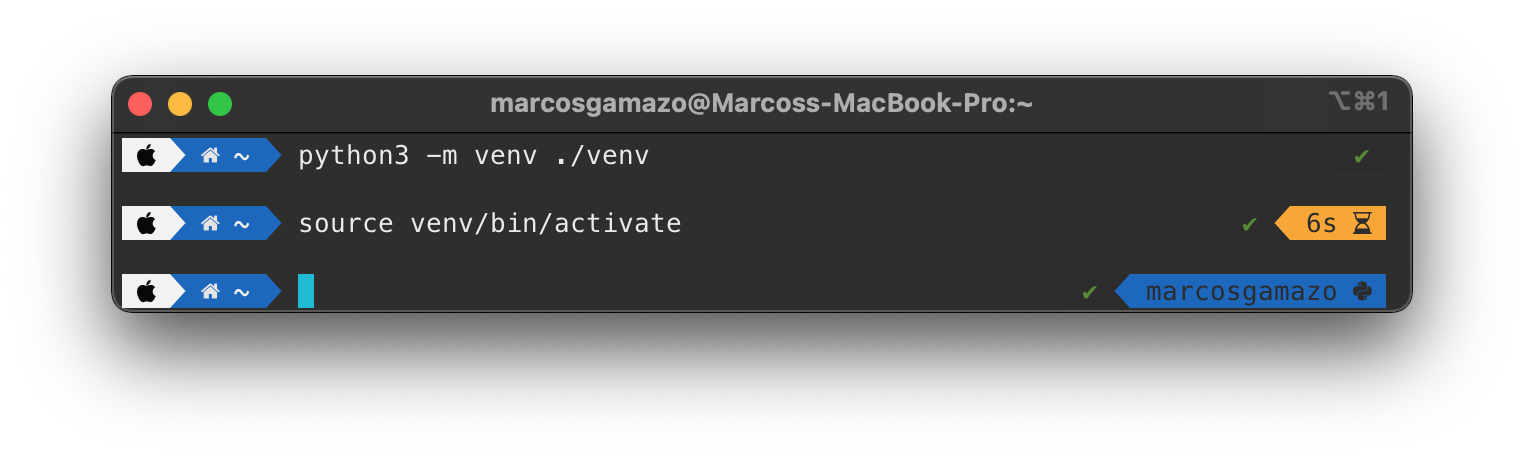
\includegraphics[scale=0.5]{include/capturas/VirtualEnv.png}
    \caption{Creación del entorno virtual}
    \label{fig:venv}
\end{figure}

Una vez creado y activado el entorno virtual procedemos a instalar Rasa mediante el comando \textit{pip3 rasa install}. Utilizamos pip3 para especificar que se instalará el framework utilizando Python 3. Cuando termine de instalarse el framework es el momento de crear la carpeta que va a contener el proyecto y acceder a ella mediante un terminal. Una vez realizado este proceso, simplemente tendremos que introducir el mandato \textit{rasa init --no-prompt}. Este mandato nos crea el bot de ejemplo de Rasa con el que se puede interactuar nada más crearlo.

Una vez tengamos la estructura creada, es hora de modificar los ficheros para que nuestro asistente se adapte a las necesidades del proyecto. Una vez modificados los distintos archivos necesarios, se debe entrenar el asistente para que cree nuestro propio modelo a utilizar para que sea capaz de comprender los mensajes que pueda introducir el usuario y que ejecute las acciones requeridas en cada momento. Para realizar el entrenamiento introduciremos en un terminal el mandato \textbf{rasa train --data data/ -c config.yml -d domain.yml --out models/}, en él se especifican los distintos archivos que tiene que utilizar para entrenar el NLU y la carpeta en la que se almacenará el modelo generado a partir del entrenamiento, como se muestra en la figura \ref{fig:rasa_train}.

\begin{figure}[H]
    \centering
    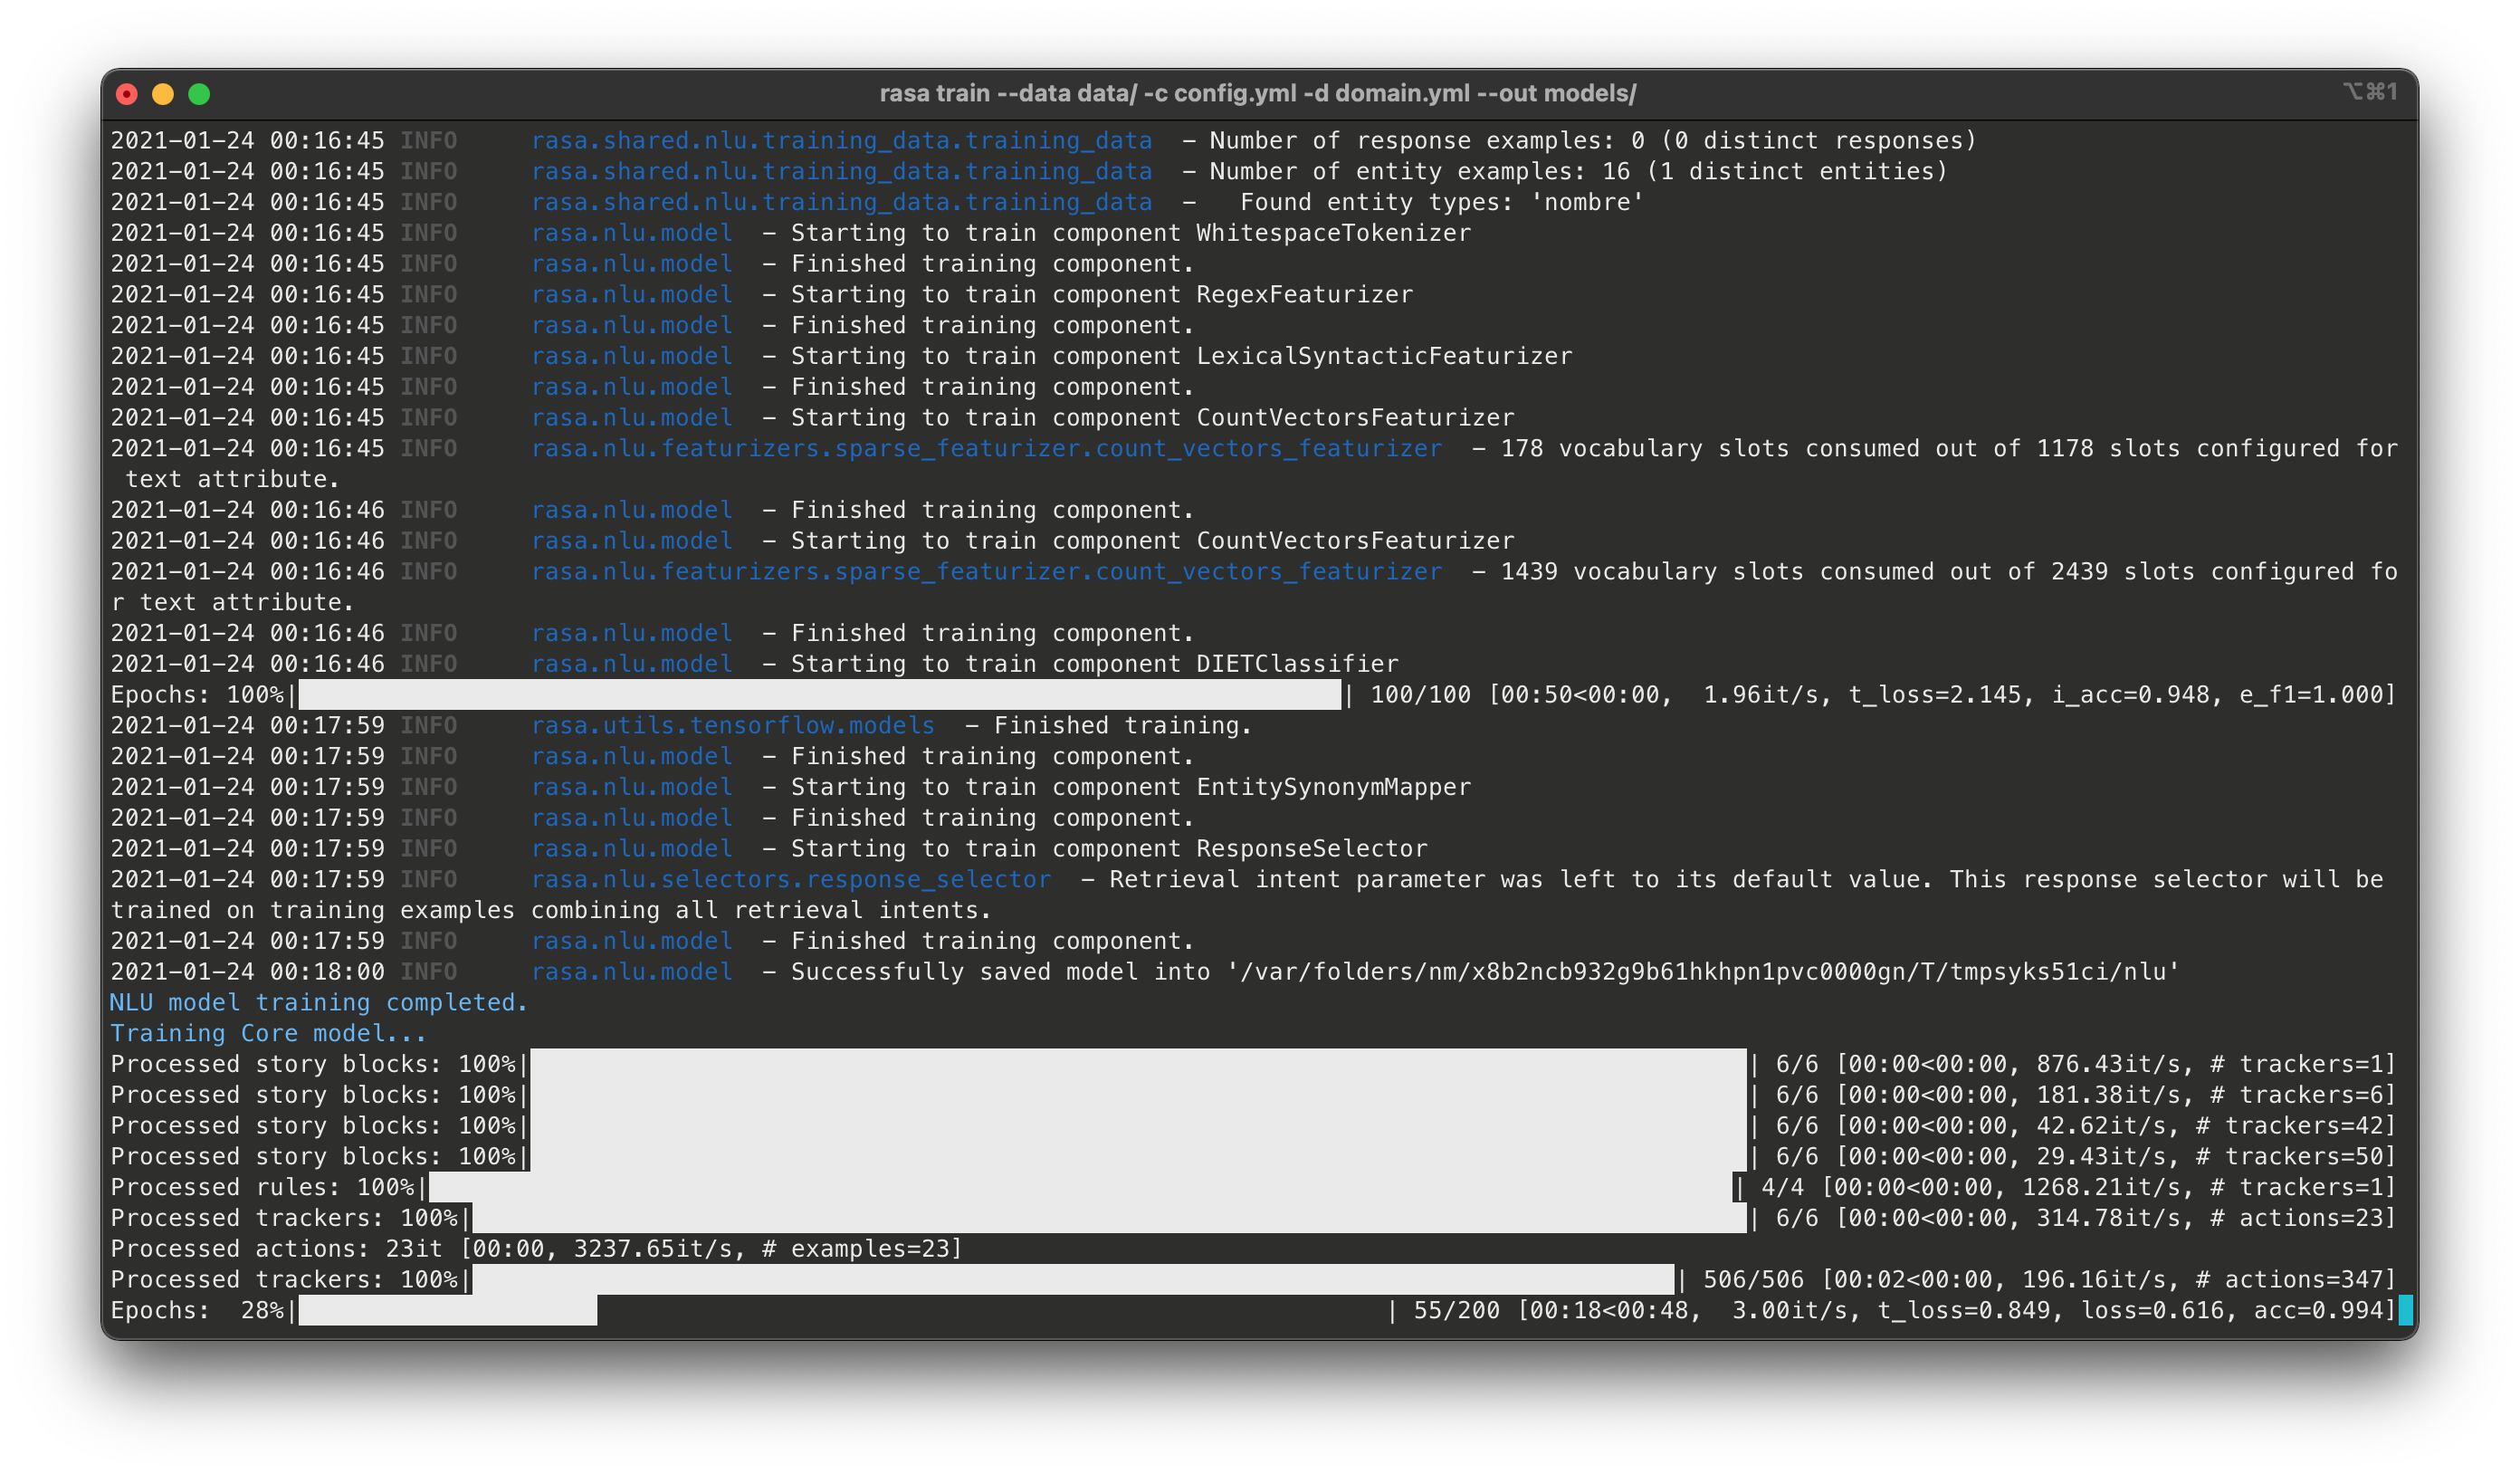
\includegraphics[width=\textwidth]{include/capturas/RasaTrain.png}
    \caption{Entrenamiento del asistente}
    \label{fig:rasa_train}
\end{figure}


Una vez realizado el entrenamiento es necesario poner en funcionamiento el servidor principal de Rasa, para ello introducimos en un terminal el comando \textbf{rasa run -m models --enable-api --cors "*"}, de esta manera le estamos diciendo a rasa qué modelo tiene que utilizar, también indicamos que se tiene que activar la API de Rasa para enviar y recibir mensajes y además activamos CORS para poder acceder a los servicios de Rasa desde un dominio diferente al de ejecución.

También es necesario activar el servidor que ejecuta las distintas acciones a realizar por el asistente, para ello se introduce el mandato \textbf{rasa run actions --actions actions -vv}. 
\newpage
\subsection{Despliegue de la base de datos y API}

La base de datos es un elemento fundamental para el funcionamiento de este proyecto pero a la vez de varios procesos paralelos en los que trabaja el equipo. Es por ello que se ha decidido realizar un despliegue mediante Docker, para reducir al mínimo las posibles incompatibilidades. 
De la mano del despliegue de la base de datos está el de la API RESTful, en nuestro caso se ha decidido realizar el despliegue de ambas herramientas de forma simultánea y en varios contenedores, aunque con la posibilidad de conectarse entre ellos.

Existen dos prerrequisitos para el despliegue de las herramientas. Por un lado, es necesaria la creación de una carpeta o de un volumen para dotar de persistencia a la base de datos, es decir, en caso de que por cualquier motivo se parase el contenedor de MongoDB, no perderíamos los datos. Y además, tener instalado \textit{Docker} dentro del sistema en el que se vaya a realizar el despliegue.

Una vez creada la carpeta, es necesario movernos hasta la carpeta donde esté ubicado el proyecto de la API RESTful y crear un fichero Dockerfile como el que se muestra en la figura \ref{fig:dockerfile} mediante el cuál vamos a especificar las distintas opciones que va a tener la imagen que creemos a partir de nuestro API creado.

\begin{figure}[H]
    \centering
    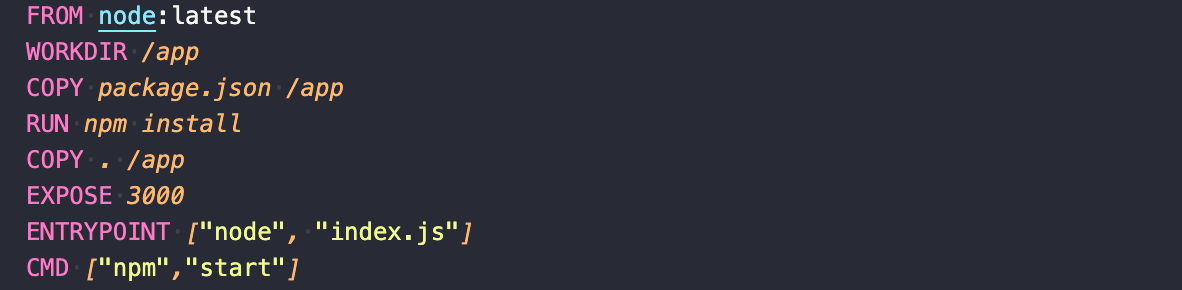
\includegraphics[width=\textwidth]{include/capturas/Dockerfile.png}
    \caption{Fichero dockerfile}
    \label{fig:dockerfile}
\end{figure}

En este fichero indicamos la imagen que hay que utilizar como base (node:latest). Para nuestra imagen, también se especifican los distintos paquetes de node.js que hay que instalar y en qué carpeta es necesario ubicarlos. Mediante el mandato \textbf{RUN npm install} se produce la instalación de dichos paquetes y con \textbf{EXPOSE 3000} indicamos el puerto en el cuál se va a poder acceder al servicio. Con el \textbf{ENTRYPOINT} decimos qué fichero va a ser nuestro ''main''. Por último, indicamos que se ejecute el comando \textbf{npm install} para poner en marcha el servicio. 

Una vez tengamos creada la imagen de nuestro API REST, crearemos el fichero docker-compose \cite{dockerCompose} mediante el cuál realizaremos el despliegue conjunto de los dos servicios, tal y como se muestra en la siguiente figura \ref{fig:docker-compose}.

\begin{figure}[H]
    \centering
    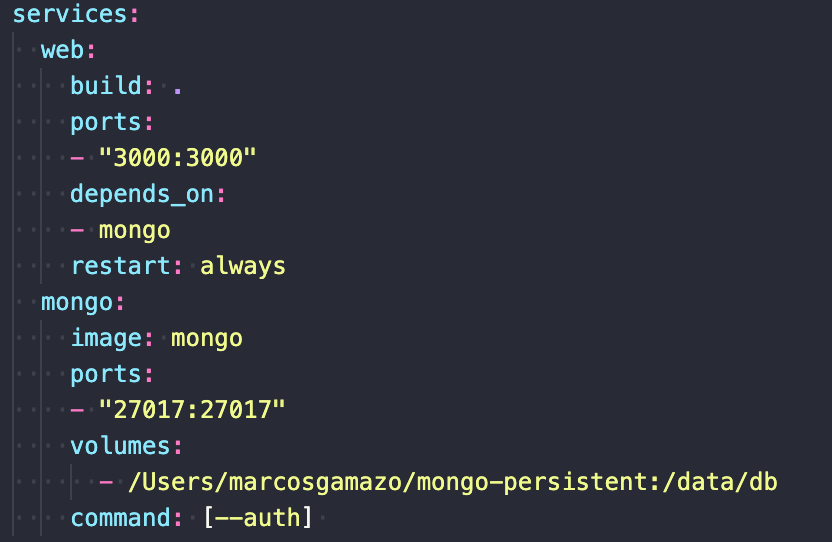
\includegraphics[width=0.75\textwidth]{include/capturas/DockerCompose.png}
    \caption{Fichero docker-compose}
    \label{fig:docker-compose}
\end{figure}

A continuación se va a proceder a la explicación de cada línea del fichero:

\begin{itemize}
    \item services: los distintos servicios que van a desplegarse mediante el docker-compose.
    \item web: servicio de la API.
    \item ''build .'': con el ''.'' le indicamos al fichero que tiene que construir el contenedor en base a la imagen que se crea en esa carpeta. 
    \item ports: puertos a exponer, a la izquierda colocamos el puerto privado y a la derecha el público.
    \item depends\_on: con esto indicamos que es obligatorio que exista un contenedor previo de mongo antes de la creación del contenedor de la API.
    \item restart: en caso de que se produzca cualquier tipo de error con el contenedor en funcionamiento, docker correrá el contenedor de nuevo automáticamente.
    \item mongo: servicio de la base de datos.
    \item image: imagen a utilizar para el contenedor de la base de datos.
    \item volumes: carpeta en la que se ubica la persistencia de la base de datos.
    \item command: comando a ejecutar una vez creado el contenedor de la base de datos, en nuestro caso, permite que se activen las autenticaciones en las diferentes bases de datos creadas dentro de MongoDB.
\end{itemize}

Una vez tengamos creado el fichero docker-compose, podemos crear ambos contenedores e iniciarlos mediante el mandato \textbf{docker-compose up -d}. Con la opción '-d' indicamos que se active el modo \textit{detached} y se ejecuten en segundo plano, como se muestra en la figura \ref{fig:dockerCompose}

\begin{figure}[H]
    \centering
    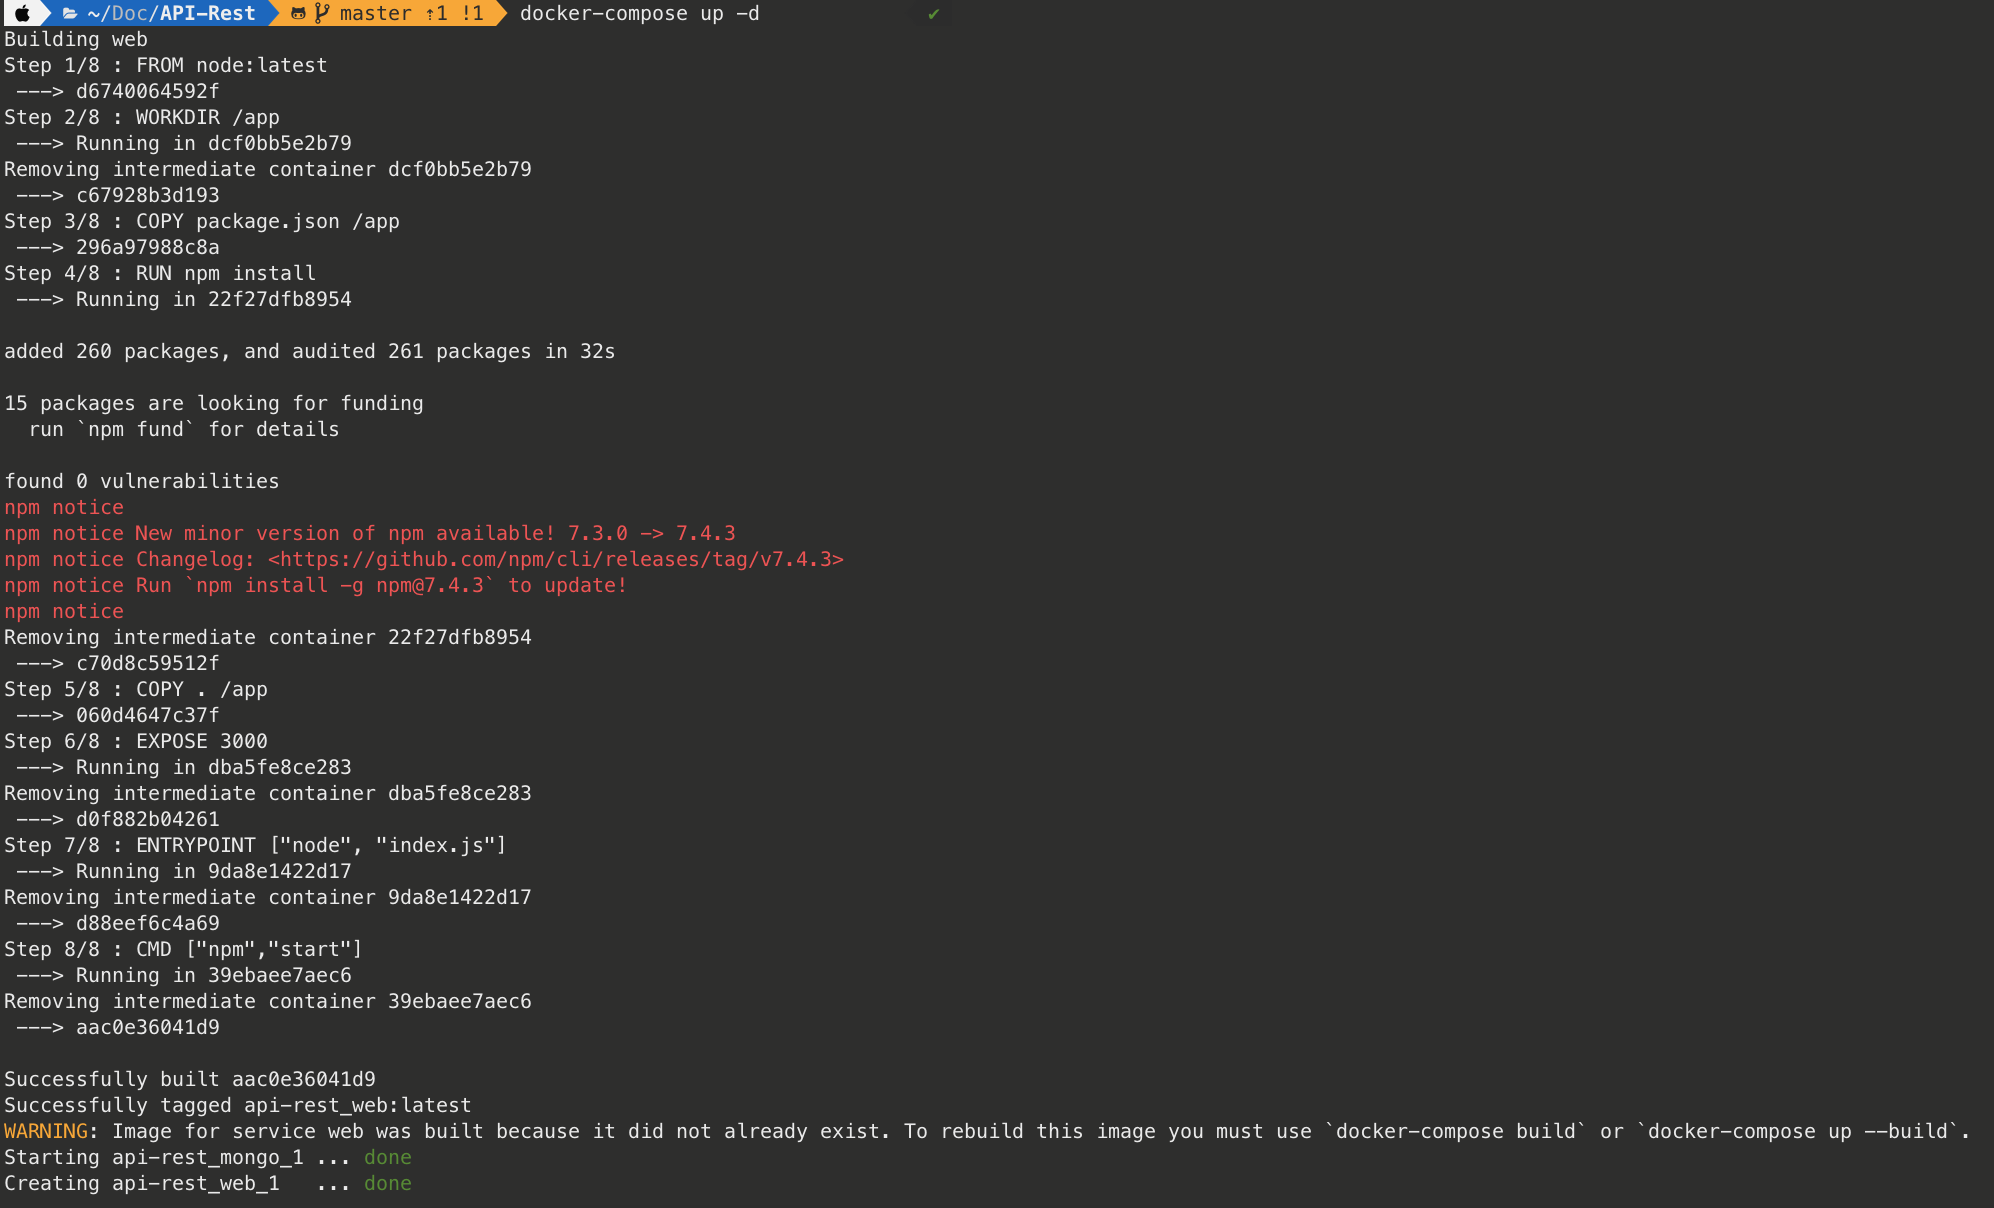
\includegraphics[width=\textwidth]{include/capturas/DockerComposeUp.png}
    \caption{Ejecución del docker-compose}
    \label{fig:dockerCompose}
\end{figure}
